\begin{exercício}{Molécula triatômica linear}{exercício1}
    Considere os estados de um elétron de uma molécula triatômica linear formada de átomos \(E, C, \) e \(D\); as distâncias \(EC\) e \(CD\) o iguais e de valor \(d\).
    \begin{center}
        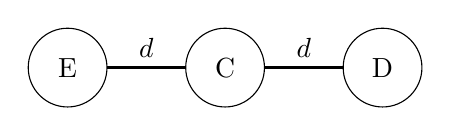
\begin{tikzpicture}
            \def\d{2}
            \draw (0, 0) circle(0.5) node at (0, 0) {E};
            \draw (\d, 0) circle(0.5) node at (\d, 0) {C};
            \draw (2*\d, 0) circle(0.5) node at (2*\d, 0) {D};
            \draw[thick] (0.5, 0) -- (\d-0.5, 0) node[midway, above]{\(d\)};
            \draw[thick] (\d+0.5, 0) -- (2*\d-0.5, 0) node[midway, above]{\(d\)};
        \end{tikzpicture}
    \end{center}
    Designamos por \(\ket{\psi_E}, \ket{\psi_C}\) e \(\ket{\psi_D}\) os autovetores normalizados do operador \(B\), correspondentes ao elétron localizado respectivamente na vizinhança dos átomos \(E, C,\) e \(D\)
    \begin{align*}
        B\ket{\psi_E} &= - d\ket{\psi_E}&
        B\ket{\psi_C} &= 0&
        B\ket{\psi_D} &= d\ket{\psi_D}.
    \end{align*}
    Quando ignoramos a possibilidade do elétron saltar de um átomo para outro, sua energia é designada pelo hamiltoniano \(H_0\) que admite como autovetores os estados \(\ket{\psi_E}, \ket{\psi_C}, \ket{\psi_D}\) com o mesmo autovalor \(E_0\). O acoplamento entre os estados \(\ket{\psi_E}, \ket{\psi_C}, \ket{\psi_D}\) é descrito por um hamiltoniano suplementar \(W\) definido por
    \begin{align*}
        W \ket{\psi_E} &= -a \ket{\psi_C}&
        W \ket{\psi_C} &= -a \ket{\psi_E} - a \ket{\psi_D}&
        W \ket{\psi_D} &= -a \ket{\psi_C},
    \end{align*}
    onde \(a > 0\).
    \begin{enumerate}[label=(\alph*)]
        \item Calcule os níveis de energia e os autoestados de \(H = H_0 + W\).
        \item Considere o estado fundamental; quais as probabilidades de encontrar o elétron em \(E, C\) e \(D\)?
        \item Considere um elétron no estado \(\ket{\psi_E}\). Se medirmos sua energia, que valores podemos encontrar? Quais as probabilidades de cada valor?
        \item Calcule o valor médio e o desvio padrão da energia para o estado \(\ket{\psi_E}.\)
    \end{enumerate}
\end{exercício}
\begin{proof}[Resolução]
    Como \(H_0 = E_0 \unity\), é claro que um vetor não nulo é autovetor de \(H\) se e somente se é autovetor de \(W\). De fato, sejam \(\ket{\lambda_W}, \ket{\lambda_H}\) autovetores de \(W\) e de \(H\) associado a autovalores \(\lambda_W\) e \(\lambda_H\), respectivamente, então
    \begin{align*}
        H \ket{\lambda_W} &= H_0 \ket{\lambda_W} + W \ket{\lambda_W}&
        W \ket{\lambda_H} &= H \ket{\lambda_H} - H_0 \ket{\lambda_W}\\
                        &= E_0 \ket{\lambda_W} + \lambda_W \ket{\lambda_W}&
                        &= \lambda_H \ket{\lambda_H} - E_0 \ket{\lambda_H}\\
                        &= (E_0 + \lambda_W) \ket{\lambda_W}&
                        &= (\lambda_H - E_0) \ket{\lambda_H},
    \end{align*}
    como afirmamos. O cômputo acima mostra ainda a relação entre os autovalores, de modo que o problema de autovalores de \(H\) é completamente determinado pelo problema de autovalores de \(W\). Notemos que
    \begin{equation*}
        W \left(\ket{\psi_E} - \ket{\psi_D}\right) = 0
        \quad\text{e}\quad
        W \left(\ket{\psi_E} \pm \sqrt{2}\ket{\psi_C} + \ket{\psi_D}\right) = \mp\sqrt{2}a\left(\ket{\psi_E} \pm \sqrt{2}\ket{\psi_C} + \ket{\psi_D}\right),
    \end{equation*}
    portanto definindo
    \begin{align*}
        \ket{0} &= \frac{1}{\sqrt{2}} \left(\ket{\psi_E} - \ket{\psi_D}\right),&
        \ket{-} &= \frac{1}{2} \left(\ket{\psi_E} + \sqrt{2}\ket{\psi_C} + \ket{\psi_D}\right),\text{ e}&
        \ket{+} &= \frac{1}{2} \left(\ket{\psi_E} - \sqrt{2}\ket{\psi_C} + \ket{\psi_D}\right)
    \end{align*}
    temos
    \begin{equation*}
        H\ket{0} = E_0 \ket{0},\quad
        H\ket{+} = (E_0 + \sqrt{2} a) \ket{+}\quad\text{e}\quad
        H\ket{-} = (E_0 - \sqrt{2} a) \ket{-}.
    \end{equation*}
    Isto é, o espectro do hamiltoniano \(H\) é dado por \(\set{E_0 - \sqrt{2} a, E_0, E_0 + \sqrt{2}a}\) e seus autoestados são \(\ket{-}, \ket{0}\) e \(\ket{+}\).

    Como estamos utilizando a base dos autovetores para o operador \(B\) de posição do elétron, a probabilidade de encontrar o elétron em \(E, C\) e \(D\) em um dado estado é justamente o quadrado do valor absoluto do coeficiente de combinação linear de \(\ket{\psi_E},\) \(\ket{\psi_C}\) ou \(\ket{\psi_D}\), uma vez que os autovalores de \(B\) são todos distintos. No estado fundamental \(\ket{-}\), essas probabilidades são dadas por \(p_E = p_D = \frac{1}{4}\) e \(p_C = \frac{1}{2}\).

    Notemos que o estado \(\ket{\psi_E}\) não é ortogonal a nenhum autoestado do hamiltoniano, portanto podemos aferir qualquer valor de seu espectro neste estado. As probabilidades \(p_-, p_0\) e \(p_+\) de medir a energia como \(E_0 - a\sqrt{2}, E_0\) e \(E_0 + a\sqrt{2},\) respectivamente, são dadas por
    \begin{align*}
        p_{-} &= \braket{\psi_E}{-}\braket{-}{\psi_E}&
        p_{0} &= \braket{\psi_E}{0}\braket{0}{\psi_E}&
        p_{+} &= \braket{\psi_E}{+}\braket{+}{\psi_E}\\
              &= \abs*{\braket{-}{\psi_E}}^2&
              &= \abs*{\braket{0}{\psi_E}}^2&
              &= \abs*{\braket{+}{\psi_E}}^2\\
              &= \frac14&
              &= \frac12&
              &= \frac14.
    \end{align*}
    Neste estado, o valor médio \(\mean{H}_{\psi_E}\) da energia é dado por
    \begin{equation*}
        \mean{H}_{\psi_E} = \bra{\psi_E}H\ket{\psi_E}
                          = \bra{\psi_E}\left(E_0\ket{\psi_E} - a\ket{\psi_C}\right) = E_0.
    \end{equation*}
    Portanto,
    \begin{align*}
        \Delta_{\psi_E}H &= \bra{\psi_E}H^2\ket{\psi_E} - \mean{H}_{\psi_E}^2\\
                         &= E_0\bra{\psi_E}H\ket{\psi_E} - a \bra{\psi_E} H \ket{\psi_C} - E_0^2\\
                         &= a^2
    \end{align*}
    é o desvio padrão \(\Delta_{\psi_E}H\) da energia.
\end{proof}

